\documentclass[a4paper,10pt]{scrartcl}
\usepackage[utf8]{inputenc}
\usepackage{enumerate,graphicx}
\usepackage[ngerman]{babel}

\begin{document}

\begin{center}
  \Huge Hardwarepraktikum \\
  \large Andre Löffler, Fabian Helmschrott, Nils Wisiol \\
  \today
\end{center}


\section*{Aufgabe C}

\section{Konfiguration}

\paragraph*{Interface-Konfiguration.} Zuerst haben wir die Interfaces der Router konfiguriert. Dazu haben wir zunächst root-Rechte mit \texttt{enable} beschafft, und anschließend mit \texttt{configure terminal} das Konfigurationsterminal geöffnet. Anschließend haben wir mit \texttt{interface FastEthernet 0/1/0} ein Interface ausgewählt und mit \texttt{ip address 10.3.1.2 255.255.255.0} ein IP-Adresse zugewiesen. Das Zuweisen einer zweiten Adresse ist mit \texttt{ip address 10.2.1.254 255.255.255.0 secondary} möglich. Nach dieser Konfiguration und mehreren \texttt{exit} war es möglich, direkte Nachbarn zu pingen.

\paragraph*{Routing-Konfiguration.} Wie oben haben wir zunächst den Konfigurationmodus geöffnet und anschließend in den Routern die statischen IP-Routen angelegt. Der Befehl dazu lautet \texttt{ip route <Ziel> <Subnetz> <Gateway>}, wobei das Gateway ein direkter Nachbar sein muss.
\begin{enumerate}
 \item[Nessos] Routing von 10.1.1.0/24 (PC-Netzwerkverkehr) über 10.3.2.2 (ate), also über exklusive Leitungen; 10.1.2.0/24 (VoIP) über 10.3.5.2 (Internet).
 \item[Styx] Routing von 10.2.1.0/24 (PC-Netzwerkverkehr) über 10.3.1.2 (ate). 10.2.2.0/24 wird ebenfalls über das Internet geroutet (Gateway: 10.3.4.2).
 \item[Ate] Ate muss Netzwerkverkehr zwischen Styx und Nessos routen, daher Routing von 10.1.1.0/24 über 10.3.1.1 (styx) und 10.2.1.0/24 über 10.3.2.1 (nessos).
\end{enumerate}
Nach dieser Konfiguration war telefonieren und pingen zwischen den Rechnern möglich. Miserable Qualität beim Telefonieren. Traceroute auf Rechner 10.2.1.1 (Distelhausen) nach 10.1.1.1 (Flensburg) ergab folgende Hops: 10.2.2.254, 10.3.2.2, 10.3.1.1, 10.1.1.1.

Zum Überprüfen der korrekten Routing-Information haben wir auf ate alle Routen gelöscht. Die PCs waren daraufhin voneinander getrennt, während die Telefone noch verbunden waren. Die Telefone mussten also die Route über das Internet nehmen.

\section{Quality-of-Service-Monitoring mit Cisco IP SLA}

\paragraph*{jitter-Konfiguration.} Zuerst haben wir auf nessos den SLA repsonder durch Eingabe von \texttt{ip sla responder} aktiviert. Anschließend haben wir auf styx den Test mit \texttt{ip sla 1}, \texttt{udp-jitter 10.3.5.1 17000}, \texttt{frequency 15} konfiguriert und mit Hilfe von \texttt{ip sla schedule 1 start-time now life forever} gestartet. Die geforderten Werte für Paketanzahl und Abstand waren voreingestellt. Anschließend können die Ergebnisse mit \texttt{ip sla statistics 1} abgerufen werden. Insgesamt haben wir 5 Messungen gestartet.

\begin{center}
  \begin{tabular}{l|rrrrr}
  Messung & 1 & 2 & 3 & 4 & 5 \\ \hline
  Messhäufigkeit (s) & 15 & 15 & 60 & 60 & 15 \\
  Paketanzahl        & 10 &100 & 10 &100 &100 \\
  Abstand (ms)       & 20 & 20 & 20 & 20 &100
  \end{tabular}
\end{center}


\paragraph*{Messergebnisse.} Die Latenz zwischen Styx und Nessos beträgt ca. 150ms. Ca. der Pakete kommt in falscher Reihenfolge an. Gelegentlich gehen Pakete verloren. Dies scheint die Ursache für die schlechte Qualität der VoIP-Verbindung zu sein, da man sich durch die hohe Latenz häufig ins Wort fällt. Änderung der Paketanzahl bzw. Messfrequenz ändert nichts an den Verhältnissen.

\section{Netzwerkmonitoring}

17:15 Uhr: gerade noch verständlich; 17:20 unverständlich.

\begin{figure}[h]
 \centering
 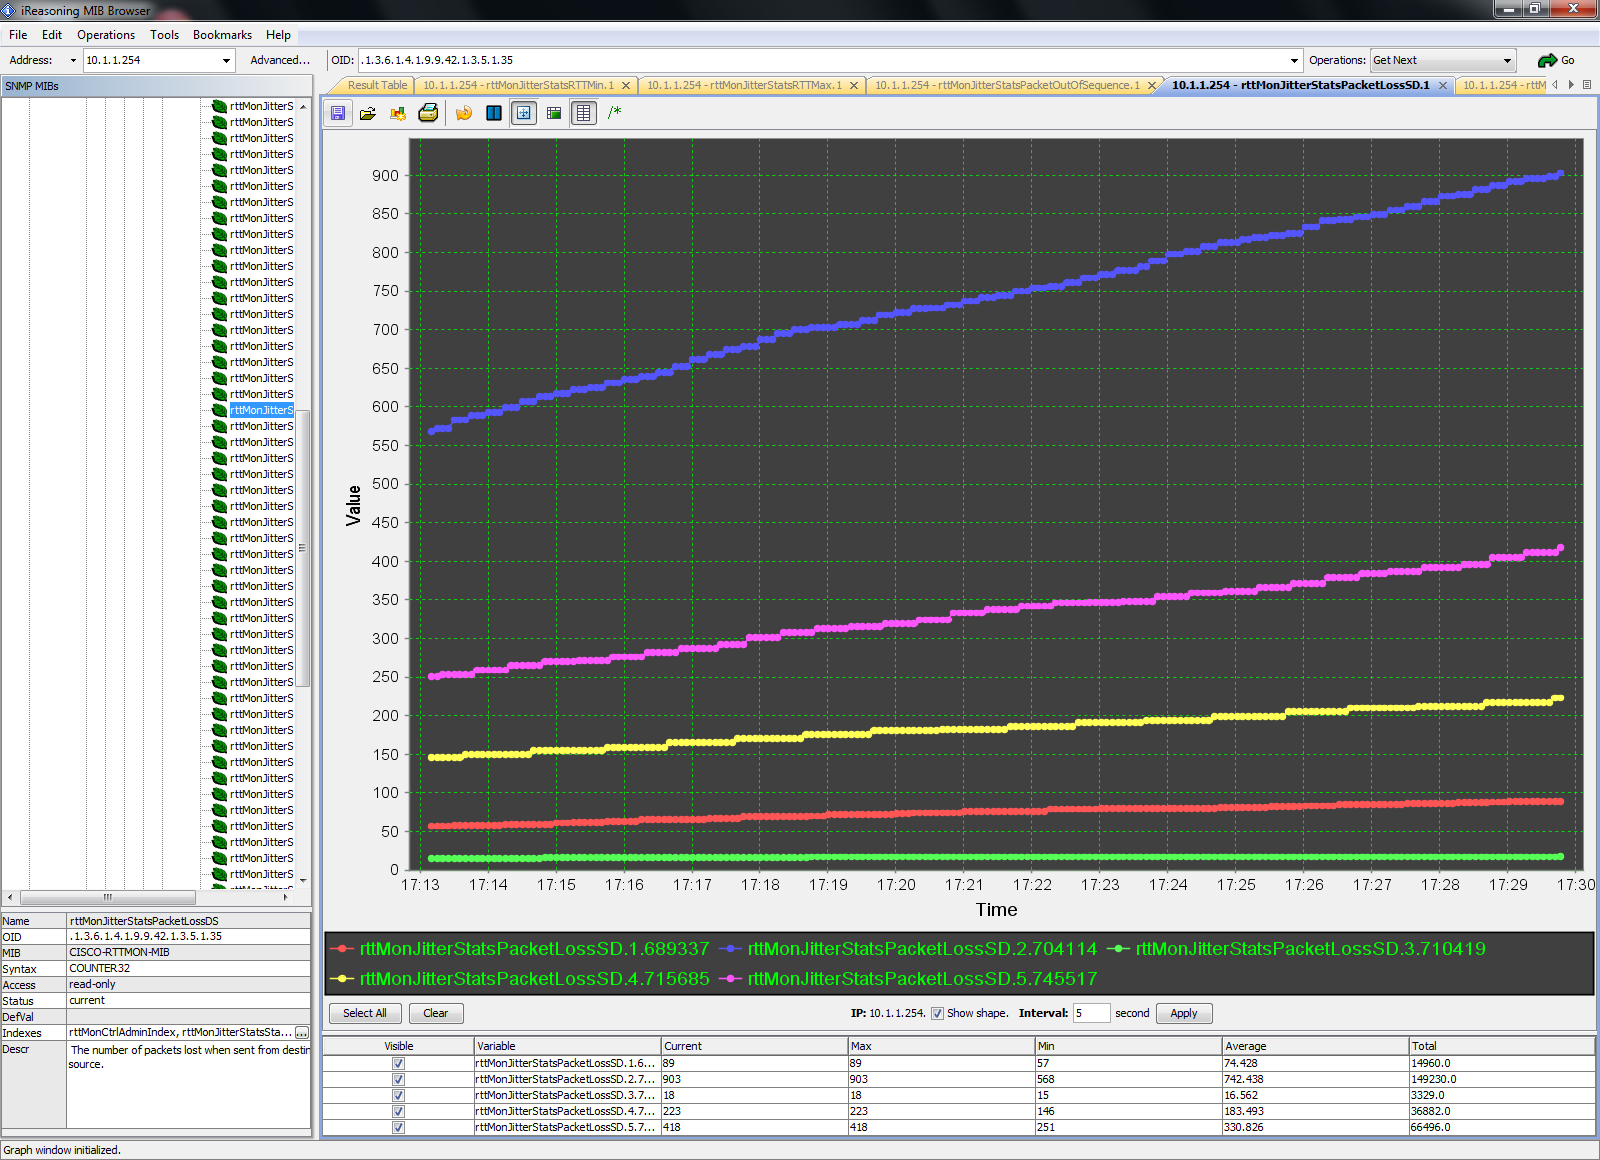
\includegraphics[width=\textwidth]{./Bilder/C/plsd.png}
 % plsd.png: 1600x1160 pixel, 96dpi, 42.34x30.70 cm, bb=0 0 1200 870
 \caption{Packet Loss Styx nach Nessos}
\end{figure}

\begin{figure}[h]
 \centering
 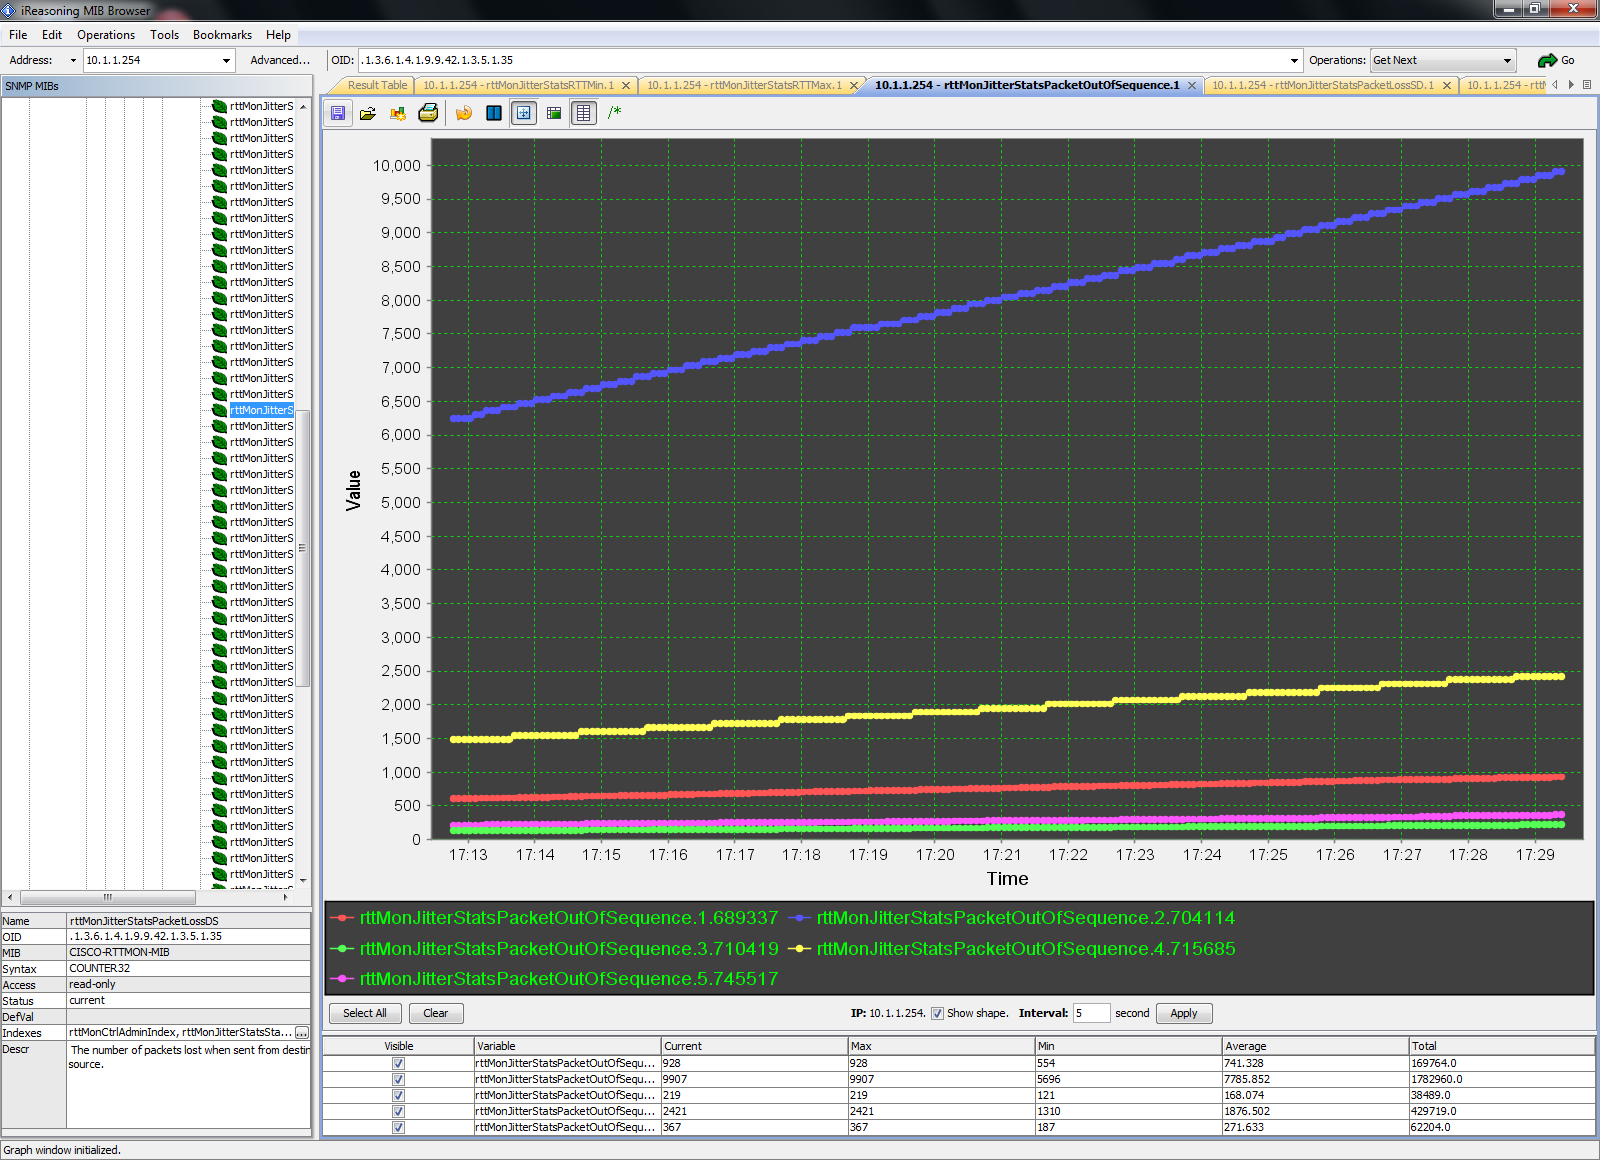
\includegraphics[width=\textwidth]{./Bilder/C/poos.png}
 % poos.png: 1600x1160 pixel, 96dpi, 42.34x30.70 cm, bb=0 0 1200 870
 \caption{Packet out of sequence}
\end{figure}

\begin{figure}[h]
 \centering
 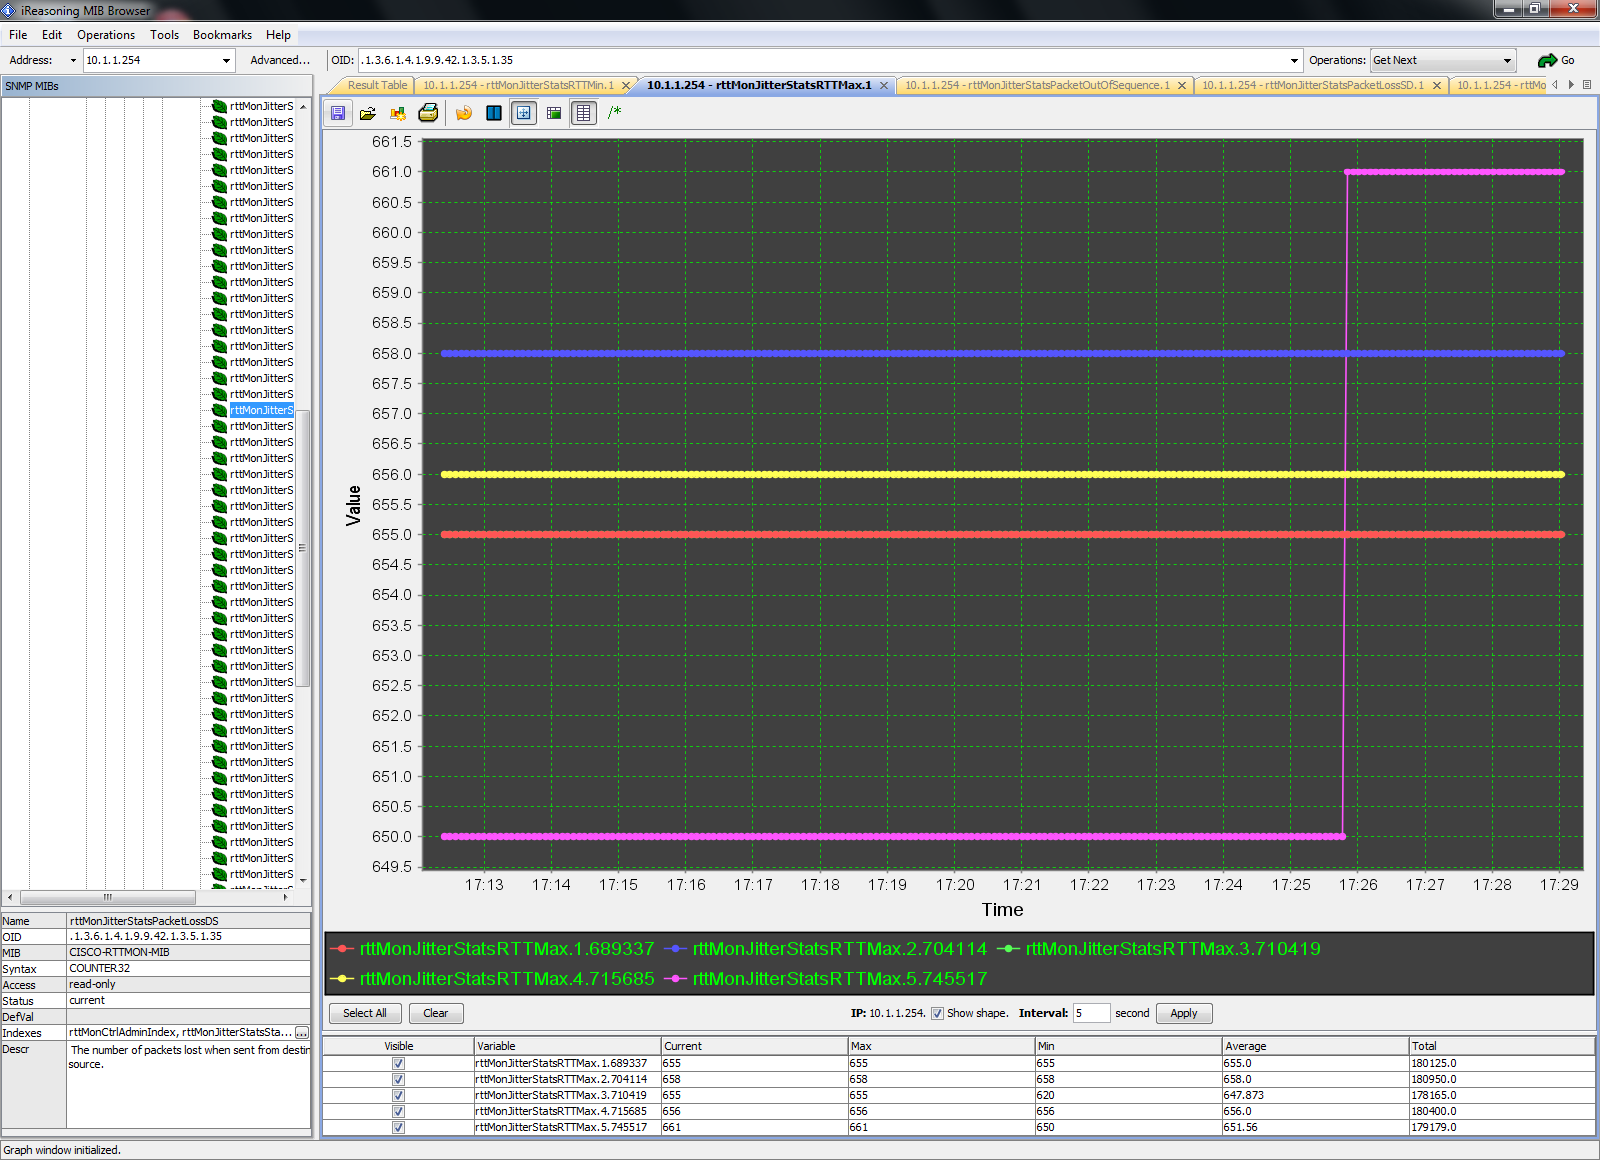
\includegraphics[width=\textwidth]{./Bilder/C/rttmax.png}
 % rttmax.png: 1600x1160 pixel, 96dpi, 42.34x30.70 cm, bb=0 0 1200 870
 \caption{Maximale RTT}
\end{figure}

\begin{figure}[h]
 \centering
 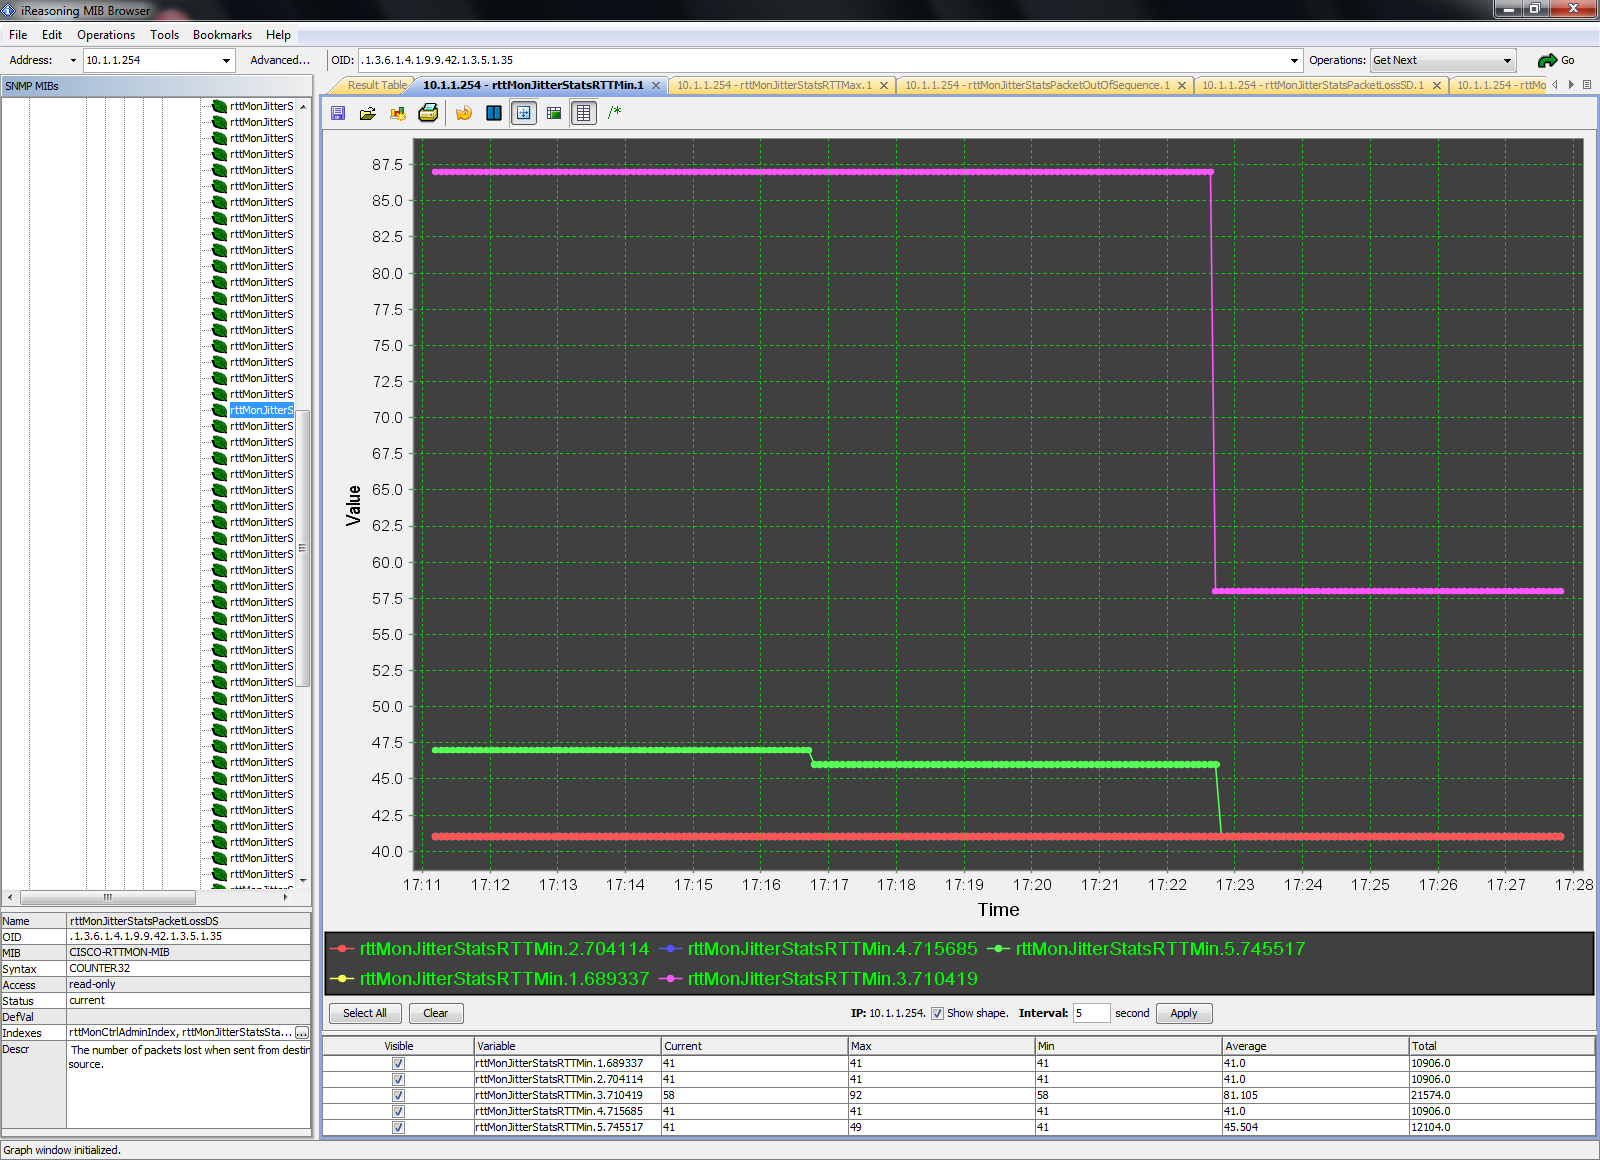
\includegraphics[width=\textwidth]{./Bilder/C/rttmin.png}
 % rttmin.png: 1600x1160 pixel, 96dpi, 42.34x30.70 cm, bb=0 0 1200 870
 \caption{Minimale RTT}
\end{figure}



\end{document}
